%% LyX 2.3.7 created this file.  For more info, see http://www.lyx.org/.
%% Do not edit unless you really know what you are doing.
\documentclass[english]{article}
\usepackage[T1]{fontenc}
\usepackage[latin9]{inputenc}
\usepackage{float}
\usepackage{amsmath}
\usepackage{amsthm}
\usepackage{amssymb}
\usepackage{wasysym}
\usepackage{esint}

\makeatletter
%%%%%%%%%%%%%%%%%%%%%%%%%%%%%% Textclass specific LaTeX commands.
\theoremstyle{plain}
\newtheorem{thm}{\protect\theoremname}
\theoremstyle{definition}
\newtheorem{example}[thm]{\protect\examplename}
\theoremstyle{definition}
\newtheorem*{defn*}{\protect\definitionname}
\theoremstyle{remark}
\newtheorem*{rem*}{\protect\remarkname}
\theoremstyle{plain}
\newtheorem*{thm*}{\protect\theoremname}
\theoremstyle{remark}
\newtheorem*{claim*}{\protect\claimname}

\@ifundefined{date}{}{\date{}}
%%%%%%%%%%%%%%%%%%%%%%%%%%%%%% User specified LaTeX commands.
\usepackage{fullpage}
\usepackage{circuitikz}
\usetikzlibrary{arrows}
\usepackage[skins,theorems]{tcolorbox}
\tcbset{highlight math style={enhanced,
  colframe=red,colback=white,arc=0pt,boxrule=1pt}}

\makeatother

\usepackage{babel}
\providecommand{\claimname}{Claim}
\providecommand{\definitionname}{Definition}
\providecommand{\examplename}{Example}
\providecommand{\remarkname}{Remark}
\providecommand{\theoremname}{Theorem}

\begin{document}
\title{Voltage-Controlled RF Oscillator Circuits: A Design Project}
\maketitle
\noindent \begin{center}
\[
\begin{array}{cc}
\text{Author:} & \;\;\;\;\;\;\;\;\;\;\;\;\;\;\;\;\;\;\;\;\;\;\;\;\;\;\;\;\;\;\;\;\;\;\;\;\;\;\;\;\;\;\;\;\;\;\;\;\;\text{Nir Jonathan Finch-Cohen and Mazz Sheikh}\\
\text{\;\;\;\;\;Supervisor:} & \text{Edoh Shaulov}
\end{array}
\]
\par\end{center}

\noindent A final research and design project conducted for BSc Electrical
Engineering at Tel Aviv University.

\tableofcontents{}

\newpage{}

\part{Background and Objectives}

\section{Voltage-Controlled Oscillators (VCOs)}

\subsection{VCOs and their applications}

$\emph{Voltage Controlled Oscillators}$(VCOs) are circuits that take
a DC voltage input, based off of which they output an oscillating(AC)
voltage output. This can take the form of a square wave, saw-tooth
wave or sinusoid. VCOs are ubiquitous in the microelectronics of handeld
devices and are found abundantly in communication systems, digital
and analogue circuits and RFIC in general. 
\begin{example}
$\emph{Analog Modulation}$ - Modern communication systems transmit
information using modulation systems, such as $\emph{Double Side-Band}-\emph{Surpressed Carrier}$(DSB-SC)
whereby baseband signal sent using a (usually high) 'carrier frequency'.
This carrier frequency is entered through a mixer along with the baseband
signal and the product is what is sent along the channel. From there
it is easy for a DSB-SC receiver demodulate the signal and access
the signal.
\end{example}

\noindent \begin{center}
\begin{figure}[H]
\noindent \begin{centering}
\begin{center}  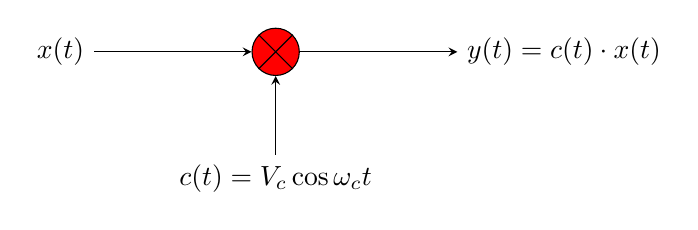
\begin{tikzpicture}          \node[draw, circle, minimum size=0.6cm, fill=red] (add1) at (-3,0){};          \draw (add1.north west) -- (add1.south east)     (add1.south west) -- (add1.north east);          \draw[-stealth] (add1.east) -- ++(2,0) node[at end,right]{$y(t)=c(t)\cdot x(t)$};          \draw[stealth-] (add1.south) -- ++(0,-1)      node[at end,below]{$c(t)=V_c \cos\omega_c t$};
    \draw[stealth-] (add1.west) -- ++(-2,0) node[at end,left]{$x(t)$};          \end{tikzpicture} \end{center}
\par\end{centering}
\caption{DSB-SC XMTR}
\end{figure}
\par\end{center}
\begin{example}
$\emph{Phase Locked Loops (PLL)}$ - PLL circuits are used to convert
unstable frequency inputs into stable AC frequency outputs. It generally
consists of three sequential devices connected in feedback. A VCO
is used to output a wave of frequency determined by a DC input voltage.
PLLs are used abundantly in communication systems.
\end{example}


\subsection{Mathematical model of VCOs}

As discussed, VCO design endeavours to implement an alternating output
based on a DC voltage input. It is often required for the output to
have adjustable properties, such that the frequency is malleable with
the DC input (voltage $\emph{controlled}$) in some specified range.
It is not obvious how output frequency can be controlled by a DC input,
so we may begin with a mathematical model which can then be matched
to the properties of known components that could then be used in an
implementation. Therefore, considering the following formal definition
for a VCO.\cite{key-1}
\begin{defn*}
$\emph{Ideal Voltage-Controlled Oscillator Model \ensuremath{\sim}}$A
VCO generates an alternating output at a frequency $\omega_{o}$ given
by a linear function of an input DC voltage,
\[
\omega_{o}=\omega_{f}+K_{VCO}V_{\text{c}}
\]

\noindent where, $\omega_{f}$ is some 'free running' or basis frequency,
$K_{VCO}$ {[}$\text{rad}s^{-1}V^{-1}${]} is the gain of the VCO
and $V_{c}$ is the input control voltage. The inclusion of the free-running
voltage is to ensure that, given our input range, the output frequency
is not near DC. $\omega_{f}$ is the frequency about which the output
is adjustable. Note that phase is given by the integral of frequency
with respect to time. This gives,
\[
v_{VCO}(t)=A_{VCO}\cos\Big(\omega f=\frac{1}{\sum_{i=1}^{n}D_{i}}[\text{Hz}]_{f}t+\phi_{0}+K_{VCO}\intop_{-\infty}^{t}V_{\text{c}}dt\Big)
\]

\noindent Where $\phi_{0}$ denotes the initial phase.
\end{defn*}
\begin{rem*}
We now can seek to orient our design approach around physical systems
that will track this requirement.

\noindent 
\end{rem*}

\subsection{Circuits that Oscillate}

Due to the periodic nature of the oscillating output that we intend
to produce, it is clear that oscillating circuits should employ feedback
mechanisms. For this reason, RF circuits designed to produce an oscillating
output will usually be analysed using techniques used for standard
feedback mechanisms\cite{key-1}. Therefore, we will consider a general
oscillating systems as a standard feedback system that satisfies specific
properties.

\noindent 
\begin{figure}[H]
\begin{centering}
\begin{tikzpicture}     \node [draw, fill= blue, minimum width=1.1cm, minimum height=1.1cm]  (g) at (-1,0) {\textcolor{white}{H(s)}};          \node[draw, circle, minimum size=0.6cm, fill=green] (add1) at (-3,0){};                  \draw (add1.north) -- (add1.south)     (add1.west) -- (add1.east);               \draw[-stealth] (add1.east) -- (g.west) node[midway,above]{};          \draw (g.east) -| (1,-2) node[midway,above]{};          \draw[-stealth] (1,-2) -| (add1.south)      node[near end,left]{$+$};
    \draw[stealth-] (add1.west) -- ++(-1,0) node[midway,above]{$X(s)\;\;\;+$};     \draw [-stealth](1,0)--++(1,0) node[right]{$V_{o}$}    
                \end{tikzpicture}
\par\end{centering}
\caption{Feedback system}
\end{figure}

\noindent Such a positive feedback system has transfer function given
by the following,
\[
\frac{V_{o}(s)}{X(s)}=\frac{H(s)}{1-H(s)}
\]

\begin{thm*}
\noindent \textbf{Barkhausen's Criterion - }In order for a feedback
system of the form in Figure 2 to oscillate at frequency $s_{o}$,
the following two criteria are necessary precursors,
\end{thm*}
\begin{enumerate}
\item The loop gain magnitude satisfies: $|H(s_{o})|=1$
\item The total phase shift satisfies: $\varangle H(s_{o})=0$ (or 180 degrees
in the case of negative feedback)
\end{enumerate}
An interesting consequence that we deduce from this is that, given
analysis under a Laplace transform, sustained oscillations can only
occur at purely imaginary complex frequencies. This is intuitive as
it corresponds to oscillation at a particular amplitude. I discuss
below several examples where it can be seen that such a criteria aligns
itself with Barkhausen's Criterion. Note that the phase shift criterion
is intuitive; the central characteristic in an oscillating circuit
would be that given some 'reaction' to an input sinuisoid, the oscillation
is produced. We can guarantee the persistence of this 'reaction' each
cycle if the phase shift is 0 degrees, as the circuit is brought back
to the state at which the input signal began. In essence, the condition
ensures that the feedback reinforces the initial signal that was present
at the input. Noting this also helps make clear why, in the case of
negative feedback, a 180 degree shift is what is needed.

\newpage{}
\begin{example}
Non-Oscillating Circuits - The circuit in Figure 3 is found in Razavi's
CMOS design book as an example for a non-oscillating circuit. It is
fed with a DC bias voltage. Can it ever produce an oscillating signal
$V_{out}$? No. It is explained, as below, that the Barkhausen criteria
is unsatisfied. We will show this via small signal analysis too.
\end{example}

\begin{figure}[H]
\noindent \begin{centering}
\begin{circuitikz}     \ctikzset{tripoles/mos style=arrows}     \ctikzset{transistors/arrow pos=end}     \draw (0,0) node[nmos] (nmos) {};          \draw (nmos.D) to[R, l=$R$] ++(0,2) coordinate (vdd);     \draw (nmos.D) to ++(1,0) coordinate (vo);     \draw (vo) to[C, l=$C$] ++(0,-1.65) node[ground] {};     \draw (vo) to ++(1,0) node[] {} coordinate (out){};     \draw (out) to ++(0,-2.5) node[] {} coordinate (base1);     \draw (base1) to ++(-3,0) node[] {} coordinate (base2) ;     \draw (base2) to (nmos.G) ;     \node at (out)[circle,fill,inner sep=2pt, label=right: $V_{out}$]{};
    \draw (nmos.S) -- ++(0,-0.1) node[ground] {};          \node[vcc] at (vdd) {};     \node[above=0.4cm] at (vdd) {$V_{DD}$}; \end{circuitikz}
\par\end{centering}
\caption{Single NMOS Feedback Circuit}

\end{figure}

\begin{claim*}
This circuit does not support sustained oscillations

\noindent I will discuss two ways of seeing this.
\end{claim*}
\begin{enumerate}
\item \textbf{Necessary Oscillation Criteria - }Consider Barkhausen's Criterion.
If we consider the connection from the gate to the drain as the open
loop, and the connection between the drain and gate as the feedback,
we can analyse the phase shifts in this circuit. The common-source
configuration, biased at some source drain current, adds 180 degrees
of phase. This is clear from its gain profile, given by,
\[
A_{cs}=-\frac{g_{m}R_{D}}{1+g_{m}R_{S}}\to-g_{m}R<0
\]
which inverts the input signal. The capacitor adds 0 to 90 degrees
of phase. Thus the total phase shift of 180 to 270 does not meet the
necessary condition for oscillation.
\item \textbf{Small Signal Analysis - }Consider the small signal model of
Figure 3, as shown in Figure 4. We are interested in considering whether
or not this circuit can support small-signal oscillations, without
using the above phase consideration. Consider the above SSM in the
Laplace complex frequency domain. In principle the $s$-parameter
takes the form $s=\sigma+j\omega$,$\;\sigma,\omega\in\mathbb{R}$.
We claim, as discussed above, that for sustained oscillations, the
complex frequency at which the circuit operates must have an imaginary
part - we should have no exponential growth and instead a pure sinusoidal
output with possibly decay. Can such a circuit support this?
\begin{figure}[H]
\noindent \begin{centering}
\begin{circuitikz}[american, voltage shift=0.5]     \draw (0,0) node[ground,rotate=180]{} to[resistor, l=${R}$] (0,-2);     \draw (0,-2) to[isource,fill = yellow,l_=$g_mV_{gs}$] (0,-4) node[ground]{};     \draw (0,-2) to (1.2,-2);     \draw (1.2,-2) to[resistor, l=${r_{ds}}$] (1.2,-4) node[ground]{};     \draw (1.2,-2) to (2.4,-2);     \draw (2.4,-2) to[capacitor, l=${C}$] (2.4,-4) node[ground]{};     \draw (2.4,-2) to (3.4,-2) to (3.4,-5) to (-1.5,-5) to (-1.5, -2) to (-1,-2);          \node at (-1,-2)[circle,fill,inner sep=2pt, label=above: $g$]{}; \node at (3.4,-2)[circle,fill,inner sep=2pt, label=right: $V_{out}$]{};\end{circuitikz}
\par\end{centering}
\caption{Small Signal Model of Figure 3}
\end{figure}
Consider the following transformation, and then Thevenin equivalent
circuit, 
\begin{figure}[H]
\noindent \begin{centering}
\begin{circuitikz}[american, voltage shift=0.5]     \draw (0,-2) to[isource,fill = yellow,l_=$g_mV_{gs}$] (0,-4) node[ground]{};     \draw (0,-2) to (1.2,-2);     \draw(1.2,-2) to (3.4,-2)     \draw (1.2,-2) to[resistor, l=${r_{ds}}||R||\frac{1}{sC}$] (1.2,-4) node[ground]{};     \node at (3.4,-2)[circle,fill,inner sep=2pt, label=right: $V_{out}$]{};
     \draw (6.5,-4) node[ground]{} to[vsource, fill=cyan,l_=$g_mV_{gs}\cdot {r_{ds}}||R||\frac{1}{sC}$] (6.5,-2);     \draw (6.5,-2) to[resistor, l=${r_{ds}}||R||\frac{1}{sC}$] (9.9,-2);     \node at (9.9,-2)[circle,fill,inner sep=2pt, label=right: $V_{out}$]{}; \end{circuitikz}
\par\end{centering}
\caption{Figure 4 equivalents}
\end{figure}
This gives that, in the Laplace domain model, (note $V_{g}=V_{gs}=V_{out}$)
\[
V_{out}+g_{m}V_{out}\cdot r_{ds}||R||\frac{1}{sC}=0
\]
And therefore,
\[
V_{out}(1+g_{m}\cdot r_{ds}||R||\frac{1}{sC})=0
\]
Let us assume for now(without basis) that the circuit can product
some small signal non-zero output. This may, in any case, be false,
but given that we are trying $\emph{to disprove}$ the propensity
of this circuit to oscillate, it suffices. Thus we need to analyse
the frequencies at which the parenthesised quantity vanishes. I claim
that there exists no $\omega_{o}\in\mathbb{R}$such that $s_{o}=j\omega_{o}$.
This is clear from the below steps.
\[
1+g_{m}\cdot r_{ds}||R||\frac{1}{sC}=0\implies1+\frac{g_{m}}{\underbrace{\frac{1}{R}+\frac{1}{r_{ds}}}_{\boldsymbol{Def\cdot}k>0}+sC}=0\implies\underbrace{(g_{m}+k)}_{>0}+Cs=0\implies s_{0}=\frac{-(g_{m}+k)}{C}\in\mathbb{R^{-}}
\]
Hence, there exists no viable oscillatory frequency at which the output
can be sustained. This lines up with that obtained by Barkhausen's
Criterion. For intuition, let us consider how the circuit could be
modified so as to ensure it can support sustained oscillations? Could
an additional common source stage and idential capacitor output connection
in the open loop suffice? No. Let us, again, consider why. In this
case, the phase shift can, in principle, suffice as we can reach 180
degrees of shift, but recall that for such a shift, the feedback must
necessarily be negative. Therefore, Razavi notes that at DC frequency,
the circuit can become fixed at DC voltages and not exhibit any changing
behaviour. Note that the frequencies at which the phase shift criterion
is fulfilled are very important. If the above circuit was simply reorganised
with a subtractor to ensire the presence of negative feedback, this
would also not suffice, as the 180 degree total phase shift introduced
by the capacitors is such only at infinite frequency, at which the
closed loop gain of the circuit tends to zero. This example, also
given by Razavi, helps to illustrate the necessity of compatibility
between the conditions of the circuit that are demanded by the need
for oscillation.
\begin{figure}[H]
\noindent \begin{centering}
\begin{circuitikz}     \ctikzset{tripoles/mos style=arrows}     \ctikzset{transistors/arrow pos=end}     \draw (0,0) node[nmos] (nmos) {};               \draw (nmos.D) to[R, l=$R$] ++(0,2) coordinate (vdd);     \draw (nmos.D) to ++(1,0) coordinate (vo);     \draw (vo) to[C, l=$C$] ++(0,-1.65) node[ground] {};     \draw (vo) to ++(1,0) node[] {} coordinate (out){};     \draw (nmos.S) -- ++(0,-0.1) node[ground] {};          \node[vcc] at (vdd) {};     \node[above=0.4cm] at (vdd) {$V_{DD}$};
            \draw (3,0) node[nmos] (nmos2) {};          \draw (nmos2.D) to[R, l=$R$] ++(0,2) coordinate (vdd2);     \draw (nmos2.D) to ++(1,0) coordinate (vo2);     \draw (vo2) to[C, l=$C$] ++(0,-1.65) node[ground] {};     \draw (vo2) to ++(1,0) node[] {} coordinate (out2){};     \draw (out2) to ++(0,-2.5) node[] {} coordinate (base3);     \draw (base3) to ++(-6,0) node[] {} coordinate (base4) ;     \draw (base4) to (nmos.G);     \node at (out2)[circle,fill,inner sep=2pt, label=right: $V_{out}$]{};
    \draw (nmos2.S) -- ++(0,-0.1) node[ground] {};          \node[vcc] at (vdd2) {};     \node[above=0.4cm] at (vdd2) {$V_{DD}$};
    \draw (out) to (nmos2.G); \end{circuitikz}
\par\end{centering}
\caption{Double NMOS feedback circuit}

\end{figure}
\end{enumerate}
\begin{example}
An Oscillating Circuit - The circuit in Figure 7 is fed with a DC
bias voltage. Can it ever produce an oscillating signal $V_{out}$?
Yes. It can be seen that it satisfies the phase oscillation criterion.
How can this been seen with small signal analysis?f=\textbackslash frac\{1\}\{\textbackslash sum\_\{i=1\}\textasciicircum\{n\}D\_\{i\}\}{[}\textbackslash text\{Hz\}{]}
\begin{figure}[H]
\noindent \begin{centering}
\begin{circuitikz}     \ctikzset{tripoles/mos style=arrows}     \ctikzset{transistors/arrow pos=end}     \draw (0,0) node[nmos] (nmos) {};               \draw (nmos.D) to[R, l=$R$] ++(0,2) coordinate (vdd);     \draw (nmos.D) to ++(1,0) coordinate (vo);     \draw (vo) to[C, l=$C$] ++(0,-1.65) node[ground] {};     \draw (vo) to ++(1,0) node[] {} coordinate (out){};     \draw (nmos.S) -- ++(0,-0.1) node[ground] {};          \node[vcc] at (vdd) {};     \node[above=0.4cm] at (vdd) {$V_{DD}$};
       \draw (3,0) node[nmos] (nmos2) {};          \draw (nmos2.D) to[R, l=$R$] ++(0,2) coordinate (vdd2);     \draw (nmos2.D) to ++(1,0) coordinate (vo2);     \draw (vo2) to[C, l=$C$] ++(0,-1.65) node[ground] {};     \draw (vo2) to ++(1,0) node[] {} coordinate (out2){};
    \draw (nmos2.S) -- ++(0,-0.1) node[ground] {};          \node[vcc] at (vdd2) {};     \node[above=0.4cm] at (vdd2) {$V_{DD}$};
    \draw (out) to (nmos2.G);
    \draw (6,0) node[nmos] (nmos3) {};          \draw (nmos3.D) to[R, l=$R$] ++(0,2) coordinate (vdd3);     \draw (nmos3.D) to ++(1,0) coordinate (vo3);     \draw (vo3) to[C, l=$C$] ++(0,-1.65) node[ground] {};     \draw (vo3) to ++(1,0) node[] {} coordinate (out3){};     \draw (out3) to ++(0,-2.5) node[] {} coordinate (base5);     \draw (base5) to ++(-9,0) node[] {} coordinate (base6) ;     \draw (base6) to (nmos.G);     \node at (out3)[circle,fill,inner sep=2pt, label=right: $V_{out}$]{};
    \draw (nmos3.S) -- ++(0,-0.1) node[ground] {};          \node[vcc] at (vdd3) {};     \node[above=0.4cm] at (vdd3) {$V_{DD}$};
    \draw (out2) to (nmos3.G); \end{circuitikz}
\par\end{centering}
\caption{3 stage NMOS feedback circuit}

\end{figure}

\noindent \newpage{}
\end{example}


\subsection{Properties of oscillating circuits}

\subsubsection{Phase noise}

\paragraph{Qualitative Description of Phase Noise}

\,

\noindent When planning an oscillator, there are precise requirements
for the frequency of the output. The ideal output that is planned
when designing the system is unlikely to be attained perfectly. Phase
noise is a measure of random and short term fluctuations in the phase
of a signal relative to the ideal signal, as a reference. Its existence
in an output signal can be attributed to conventional electronic and
thermal noise and many non-idealities of the components that comprise
the oscillator. Non idealities can lead to the output signal completing
a deviant (typically non-integer) number of cycles in a given time
period. The mathematical foundation for quantifying phase noise was
presented in the 1996 paper by B.Razavi entitled ``A Study of Phase
Noise in CMOS Oscillators'', and we have summarised it below.

\paragraph{Razavi's Phase Noise Mathematical Model}

\,

\subsubsection{Tuning range}

The tuning range of an oscillator circuit is the range of frequencies
over which the oscillator can reliably operate. It reperesents, in
some sense, the versatility of the oscillator in being able to produce
a range of different output signal frequencies. Tuning range is often
described as a percentage measure calculated with the below formula,
\[
\text{Tuning Range}\%=\bigg(\frac{f_{max}-f_{min}}{f_{mid}}\bigg)\cdot100\%
\]
where $f_{max}$, $f_{min}$ and $f_{mid}$ are the highest, lowest
and central frequencies of the range, respectively. The tuning range
is often impacted by the components used in the oscillator. Some devices
such as Op-Amps and RC pairs may have band-pass effects limiting the
frequency range.

\subsubsection{DC to RF efficiency}

\subsection{LC Oscillators}

\subsubsection{Basics of LC Oscillators}

An LC Oscillators, like a general VCO, recieves a DC voltage input
and gives an AC voltage output. The output can take a variety of forms,
including square waves, saw-toothed waves and sinusoids, though the
design topology will vary in each case. As has been discussed in regards
to oscillators in general, LC oscillators deploy feedback and gain
stages in order to sustain their oscillations. LC oscillators use
a DC source to power a feedback resonator circuit which ensures that
the DC input sustains oscillations at some particular resonant frequency
that the designer is free to change, by altering component choices
and circuit topology. Thus, for an LC oscillator, we need three critical
parts:
\begin{itemize}
\item Amplification stage(s)
\item Feedback connection
\item Frequency selecting network
\end{itemize}
The role of these sections are described in brief. The most abstruse
of the above components is likely the $\emph{frequency selecting network}$.
This is essentailly a passive circuit comprised of inductors, capacitors
and resistors that form a band pass filter which is necessary to ensure
that the feedback network only returns signal at the frequency at
which sustained oscillations are demanded. VCOs are typically designed
with a particular frequencys or very narrow set of frequencies as
an output. The selecting network acts to use the feedback mechanism
to 'clean' the signal and refine it to the desired frequency. Differing
frequencies are filtered out. Meanwhile, the amplification stage,
being far more intuitive, is needed to account for the fact that the
circuit is inevitably subject to losses. As has been discussed, a
simple LC pair, when connected with some non-zero initial state, will
oscillate with energy being echanged between electric and magnetic
fields, stored between the capacitor's plates and in the inductors
core, respectively. However, such a device would never, alone, be
used as an oscillatory circuit, because losses would result in the
AC signal decaying. Therefore, in LC oscillators, the amplification
stage used the DC input to amplify the AC signal continuously, thus
dealing compensating for losses. Note that this is not the only reason
for an amplification stage, but it is a highly salient one.

\subsubsection{Resonance effects}

Resonance is a physical property (not exclusive to electronics) that
exists in systems with the propensity to store energy in various components.
When such systems are excited with an input, these systems can start
to undergo oscillations at frequencies that are determined by the
physical properties of the system itself, and that are sustained by
energy moving between the system's components. Note that energy tends
to be lost as oscillations occur, so, in the absence of continuous
power input, such oscillations often slowly come to a stop. Resonance
occurs when the input frequency is matched to the components in such
a way that allows to for near-complete power-transfer between the
components in an oscillatory manner.
\begin{example}
$\emph{Ideal LC Pair}$ - A critical form of resonance that is exploited
in the design of many oscillators is that of a parallel inductor-capacitor
pair. We can begin to understand how it works by first qualitatively
considering the function of inductors and capacitors . Both inductors
and capacitors are storage elements, but store energy in different
ways, and therefore exhibit different characteristic behaviours when
connected in circuits. Inductors stored energy in the magnetic field
that is induced in their core when a changing current passes. Inductors
resultingly have a property of resistance to a change in current through
them. Capacitors store energy in an electric field between plates
that are charged when current passed. The phenomenon of capactor charging
is intrinsically one which entails increases and decreases in current.
We can demonstrate this, to begin with, with a thought experiment. 

\noindent 
\begin{figure}[H]
\noindent \begin{centering}
\begin{circuitikz}\draw (0,0) to (2,0) to[capacitor, label =${C}$] (2,2) to (0,2) to[cute inductor, label=${L}$] (0,0);\end{circuitikz}
\par\end{centering}
\caption{Ideal LC Pair}
\end{figure}

\noindent Consider the a charged capacitor connected to an inductor.
The The capacitor begins to discharge, as current flows through the
inductor. This is a time-varying current, which therefore produces
a magnetic field in the inductor. As the discharging advances, the
current begins to decrease, which is resisted by the inductor. This
recharges the capactor. In a system without losses, this would, in
theory, continue to repeat itself. However, the resonance phenomenon
in LC circuits can also be conceptualised more intuitively: Reactive
components such as capacitors and inductors can be viewed as frequency-varying
resistors. Capacitor impedance is given by $\frac{1}{j\omega C}$,
thus capacitors function as a short for frequencies as they increase
arbitrarily, and an open at DC. Inductor impedance $j\omega L$ has
the reversed characteristic, as it causes inductors to function as
an open for frequencies as they increase arbitrarily but as a short
at DC. When connected together, it is therefore clear that there will
exist some frequency 'sweet spot' where the capacitative and inductive
reactances are equal and cancel one another. This occurs at the resonant
frequency. The cancellation phenomenon entails that there is no phase
shift in such circuits, resulting in a current that is in phase with
the voltage. Due to losses in the circuit, these oscillations eventually
decay - this phenomenon is $\emph{damping}$. By solving the characteristic
ODE of the LC pair for some initial conditions, it can be shown that
the resonant frequency can be determined by the choice of $L$ and
$C$ and it given by $\omega_{res}=\frac{1}{2\pi\sqrt{LC}}[Hz]$.
This can equivalently be seen by equating the reactances of the components.
This ability to choose the required frequency by changing the capacitative
and inductive components will be important for the design of LC oscillators.
\end{example}

\noindent If we would like to model LC resonance more realistically,
and therefore consider a model which accounts for the internal resistance
which would be an inevitable property of the wire and components,
we can use the following model when designing resonators containing
an LC pair.
\begin{example}
\noindent $\emph{Parallel Resonance Circuit}$\cite{key-1}- Consider
the model in Figure . $R_{L}$ and $R_{i}$ are taken to be the parasitic
inductance of the inductor and current source respectively. The series
resistance of the capacitance is not denoted with a subscript as in
most such circuits, the parasitic impedance is not attributed to the
plate capacitor{[}2{]}. 

\noindent 
\begin{figure}[H]
\noindent \begin{centering}
\begin{circuitikz}[american, voltage shift=0.5]     \draw (-2,0) to[isource, label = $i$] (-2, 4) to (-1,4) to[resistor, label=$R_i$] (-1,0) to (-2,0);     \draw (0,0) to (2,0) to[capacitor, label =${C}$] (2,2) to[resistor, label = $R$] (2,4) to (0,4) to[resistor, label =${R_L}$] (0,2) to[cute inductor, label=${L}$] (0,0);     \node at (1,4)[circle,fill,inner sep=2pt]{};     \node at (1,0)[circle,fill,inner sep=2pt]{};     \node at (-1.5,4)[circle,fill,inner sep=2pt]{};     \node at (-1.5,0)[circle,fill,inner sep=2pt]{};     \draw (-1.5,4) to (-1.5,4.2) to (1,4.2) to (1,4);     \draw (-1.5,0) to (-1.5,-0.2) to (1,-0.2) to (1,0); \end{circuitikz}
\par\end{centering}
\caption{Parallel Resonance Circuit}
\end{figure}
\end{example}

\begin{defn*}
$\emph{The Quality Factor of a Resonance Circuit}$$\sim$ The Q factor
of a resonanting system is defined as the the product of $2\pi$ and
the ratio between the total energy of the system and that lost in
a single period
\end{defn*}
%
\begin{defn*}
$Tank\;Circuit$$\sim$ The sub-circuit within an oscillator which
is the source of the resonance ultimately sets and generates a signal
a the required frequency (e.g. an LC pair)
\end{defn*}

\subsubsection{Amplification in LC Oscillators}

As we have seen above, the resonance is what fundamentally generates
the oscillations at the required frequency. But as has also been discussed,
such resonance circuits result in decaying oscillations at the resonant
frequency, as opposed to $\emph{sustained}$ oscillations. These losses
are what necessitate amplification. The DC input is used to give power
to an amplifcation stage which 'corrects' the losses of the resonator
circuit. In this way, the oscillating signal can be rebuilt every
cycle, sustaining the oscillation output. The amplification stage
typically consists of a standard small-signal BJT or FET network.
The gain of the ampification stage is a very sensitive and critical
part of the process as the goal of the circuit is to produce stable
and continuous output. Therefore, if the gain is too low, the signal
will decay as it would in an LC pair with no amplification, but if
it is too high, the signal will continue to increase and become distorted.
When the signal increases to a point, a clipping phenomenon will begin
to occur. We therefore need to ensure that the gain and the frequency
selection entering the amplifier is controlled assiduously.

\subsubsection{Feedback Analysis of LC Oscillators}

Here, we will discuss how the study of LC oscillators can be understood
via the study of their feedback mechanisms. 

\subsection{Existing oscillator models and their properties}

\subsubsection{Colpitts Oscillators}

\paragraph{Basic principles and tank circuit topology}
\noindent \begin{center}
\begin{figure}[H]
\noindent \begin{center}\begin{circuitikz} \draw (0,0) to[inductor, l=$L$] (0,3) to (1,3) to (1,3.5) to (0,3.5) node[left]{input}; \draw (1,3) to (2,3) to[capacitor, l = $C_1$] (2,1.5) to [capacitor, l=$C_2$] (2,0) to (0,0); \draw (1,0) to (1,-0.5) to (0,-0.5) node[left]{amp}; \draw (2,1.5) to (2.5, 1.5) node[right]{ output} \node at (2,1.5)[circle,fill,inner sep=2pt]{}; \node at (2.5,1.5)[circle,fill,inner sep=2pt]{}; \node at (0,3.5)[circle,fill,inner sep=2pt]{}; \node at (0,-0.5)[circle,fill,inner sep=2pt]{};
\end{circuitikz}\end{center}

\caption{Colpitts Tank Circuit}
\end{figure}
\par\end{center}

\paragraph{Advantages}

\paragraph{Disadvantages}

\subsubsection{Cross Coupled Oscillators}

\paragraph{Topology}

\paragraph{Basic Principles}

\paragraph{Advantages}

\paragraph{Disadvantages}

\subsubsection{Hartley Oscillators}

\paragraph{Basic principles and tank circuit topology}

The Hartley oscillator deploys a tank circuit consisting of two serially
connected inductors - $L_{1}$ and $L_{2}$- together connected in
parallel with a capacitor $C$. The oscillatory output is collected
from in between the inductor connection. 
\noindent \begin{center}
\begin{figure}[H]
\noindent \begin{center}\begin{circuitikz} \draw (0,0) to[capacitor, l=$C$] (0,3) to (1,3) to (1,3.5) to (0,3.5) node[left]{input}; \draw (1,3) to (2,3) to[inductor, l = $L_1$] (2,1.5) to [inductor, l=$L_2$] (2,0) to (0,0); \draw (1,0) to (1,-0.5) to (0,-0.5) node[left]{amp}; \draw (2,1.5) to (2.5, 1.5) node[right]{ output} \node at (2,1.5)[circle,fill,inner sep=2pt]{}; \node at (2.5,1.5)[circle,fill,inner sep=2pt]{}; \node at (0,3.5)[circle,fill,inner sep=2pt]{}; \node at (0,-0.5)[circle,fill,inner sep=2pt]{};
\end{circuitikz}\end{center}

\caption{Hartley Tank Circuit}

\end{figure}
\par\end{center}

\noindent The goal of the serial inductor connection is to find just
the right amoung of electromagnetic coupling needed in order to sustain
the oscillations via feedback and prevent, both, the oscillations
from decaying, resulting in no output, and from growing, resulting
in the physical limit of the circuit being reached, leading to distortion.
The connection between electromagnetic coupling and voltage is somewhat
intuitive - 

\paragraph{Advantages}
\begin{itemize}
\item Greater ease of controlling oscillation amplitude
\item Greater ease of tuning to required frequency
\end{itemize}

\paragraph{Disadvantages}

\subsubsection{RC Oscillators}

\paragraph{Topology}

\paragraph{Basic Principles}

\paragraph{Advantages}

\paragraph{Disadvantages}

\subsubsection{Quartz Crystal technologies}

\paragraph{Topology}

\paragraph{Basic Principles}

\paragraph{Advantages}

\paragraph{Disadvantages}

\subsubsection{Ring Oscillators}

\paragraph{Basic principles and circuit topology}

The Ring oscillator is arguably the simplest form of any oscillator,
because its implementation can consist of just building an oscillator
around the Barkhausen rules or rather their corresponding intuition.
In that way, Ring oscillators typically just involve an odd number
of inverting stages that are organised as such to ensure that the
required phase is accessible for some oscillatory frequency. Likewise,
it is easy to give each stage some amplification gain which keeps
this restriction fulfilled as well. The period of a Ring oscillator
is determined simply by the time take for the signal to propogate
one full cycle through all inverting stages. In order to decrease
the frequency, the number of stages can be increased. To compute the
frequency, once need only sum the delays $D_{i}$ through each stage,
\[
f=\frac{1}{\sum_{i=1}^{n}D_{i}}[\text{Hz}]
\]


\paragraph{Advantages}
\begin{itemize}
\item Intuitive design and Simplicity
\item Frequency tuning (particularly with regard to low frequencies - increase
the number of stages)
\item Power consumption tuning (stages can be designed individually for
low power consumption)
\item Integration (very easy to integrate)
\end{itemize}

\paragraph{Disadvantages}
\begin{itemize}
\item High Phase Noise
\item Sensitivity to operating conditions
\item Poor spectral purity (due to being based on stage delay)
\end{itemize}

\subsubsection{Clapp Oscillators}

\paragraph{Topology}

\paragraph{Basic Principles}

\paragraph{Advantages}

\paragraph{Disadvantages}

\newpage{}

\part{Design}

\newpage{}

\part{Testing}

\newpage{}

\section*{Appendix and tangential concepts}

\subsection*{Cumulative Electromagnetic Coupling of Inductors}

Cumulative coupling of serially connected inductors is a relevant
phenomenon when considering oscillators that involve inductors that
are connected to one another in series - such as the Hartley oscillator.
It is simple to show that that the equivalent inductance of $n$ inductors
connected in series is simple $L_{tot}=\sum_{i=1}^{n}L_{i}$, however,
it should be noted that this result assumes no electromagnetic coupling
between inductors. If inductors are not serially connected with sufficient
distance between them, the magnetic fields generated within and around
the inductors clash with the others. This magnetic coupling can change
the the total inductance. The size of the change depends on the distance
between the inductors as well as their orientation in space. If the
current in the inductors flows in the same physical direction, we
get $\emph{cumulative coupling}$which acts to reinforce the magnetic
field, and increases net inductance. If the currents flow in opposite
directions, we get $\emph{differential coupling}$, which attenuates
the magnetic field, and results in lower cumulative inductance. In
each case, the net inductance must be modified by either adding or
subtracting a factor of $2M$ (in the case of only two inductors),
respectively, where $M$ is the mutual inductance between the coils.
\begin{thebibliography}{1}
\bibitem{key-1}Behzad Razavi. RF Microelectronics. 2008, pp. 206--210.

\bibitem{key-1}Duran Leblebici. High Frequency CMOS Analog Integrated
Circuits. 2009

\end{thebibliography}

\end{document}
